% Simple Sectioned Essay Template
% LaTeX Template
%
% This template has been downloaded from:
% http://www.latextemplates.com
%
% Note:
% The \lipsum[#] commands throughout this template generate dummy text
% to fill the template out. These commands should all be removed when 
% writing essay content.
%
%%%%%%%%%%%%%%%%%%%%%%%%%%%%%%%%%%%%%%%%%

%----------------------------------------------------------------------------------------
%	PACKAGES AND OTHER DOCUMENT CONFIGURATIONS
%----------------------------------------------------------------------------------------

\documentclass[12pt]{article} % Default font size is 12pt, it can be changed here

\usepackage{geometry} % Required to change the page size to A4
\geometry{a4paper} % Set the page size to be A4 as opposed to the default US Letter

\usepackage{graphicx} % Required for including pictures
\usepackage[utf8]{inputenc}
\usepackage{float} % Allows putting an [H] in \begin{figure} to specify the exact location of the figure
\usepackage{listings}
\usepackage{float}
\renewcommand{\contentsname}{Sisällysluettelo}
\linespread{1.2} % Line spacing

%\setlength\parindent{0pt} % Uncomment to remove all indentation from paragraphs

\graphicspath{{./Pictures/}} % Specifies the directory where pictures are stored

\begin{document}

%----------------------------------------------------------------------------------------
%	TITLE PAGE
%----------------------------------------------------------------------------------------

\begin{titlepage}

\newcommand{\HRule}{\rule{\linewidth}{0.5mm}} % Defines a new command for the horizontal lines, change thickness here

\center % Center everything on the page

\textsc{\LARGE Helsingin Yliopisto}\\[1.5cm] % Name of your university/college
\textsc{\Large Tietojenkäsittelytieteen laitos}\\[0.5cm] % Major heading such as course name
\textsc{\large Tietokantasovellus}\\[0.5cm] % Minor heading such as course title

\HRule \\[0.4cm]
{ \huge \bfseries AC Hannes Statistics Tool}\\[0.4cm] % Title of your document
\HRule \\[1.5cm]

\begin{minipage}{0.4\textwidth}
\begin{flushleft} \large
\emph{Tekijä:}\\
Ilkka \textsc{Hakkarainen} % Your name
\end{flushleft}
\end{minipage}
~
\begin{minipage}{0.4\textwidth}
\begin{flushright} \large
\emph{Ohjaaja:} \\
Harri \textsc{Laine} % Supervisor's Name
\end{flushright}
\end{minipage}\\[4cm]

{\large \today}\\[3cm] % Date, change the \today to a set date if you want to be precise

%\includegraphics{Logo}\\[1cm] % Include a department/university logo - this will require the graphicx package

\vfill % Fill the rest of the page with whitespace

\end{titlepage}

%----------------------------------------------------------------------------------------
%	TABLE OF CONTENTS
%----------------------------------------------------------------------------------------

\tableofcontents{Sisällysluettelo} % Include a table of contents

\newpage % Begins the essay on a new page instead of on the same page as the table of contents 

%----------------------------------------------------------------------------------------
%	INTRODUCTION
%----------------------------------------------------------------------------------------

\section{Esittely} % Major section
AC Hannes Statistics Tool on urheilulajisitomaton tilastointijärjestelmä, joka mahdollistaa äärimmäisen dynaamisen tilastoinnin ja tilastojen koostamisen. Tuettuja ominaisuuksia ovat mm. uusien tilastoitavien artikkelien lisääminen lennosta ja tilastojen koostaminen esimerkiksi pelikentän tai vastustajajoukkueen mukaan. Innostus aiheeseen tuli omasta ja jalkapallojoukkueen tarpeesta tuoda toiminta seuraavalle vuosituhannelle. Tilastointipalvelu käyttää yhteistä tietokantaa AC Hanneksen kotisivujen kanssa, joten osa määrittelyistä voi tuntua epäolennaiselta sovelluksen kannalta ja niitä ei myöskään käsitellä sen tarkemmin tässä dokumentissa.
%------------------------------------------------

\subsection{Käytetyt tekniikat} % Sub-section
Sovellus on rakennettu toimimaan PostgreSQL-kannan päällä ja se koostuu yksinkertaisista php-skripteistä. Näillä ratkaisuilla pyritään takaamaan Statistics Toolin helppo siirrettävyys ja laajennettavuus.


%------------------------------------------------

\section{Ohjelman rakenne} % Sub-section
Käyttöliittymältään AC Hannes Statistics Toolilla on kaksi tilaa, jotka heijastavat suoraan eri käyttäjäkuntia. Koostamistilassa käyttäjän on mahdollista käsitellä tietokannan tietoja read-only tilassa, jolloin käyttäjän päätavoitteena on monipuolisen tilastodatan koostaminen erilaisiin tarkoituksiin. Joukkueen johtoportaalle tarjotaan sen sijaan elegantti ja helppokäyttöinen käyttöliittymä tilastojen luomiseen ja poistamiseen, sekä tilastoartikkelien päivittämiseen. Kaiken tämän dynaamisen toiminnan mahdollistaa tietokannan rakenne, joka perustuu useaan yksinkertaiseen tauluun, joista voidaan johtaa monimutkaisia tilastotietoja.
%------------------------------------------------

\subsection{Tietokannan rakenne ja määrittely} % Sub-sub-section
\lstset{frame=single, language=SQL, caption=Create Table Statements, basicstyle=\footnotesize, breaklines=true,}
\begin{lstlisting}
CREATE TYPE RESULT AS ENUM ('w', 't', 'l');
CREATE TYPE PLATFORM AS ENUM ('nurmi', 'hiekka', 'tekonurmi', 'sisä', 'laivan kansi');

/*
* EI CASCADEA, jos pelaaja poistetaan. Muuten lopputulos muuttuu.
*/
CREATE TABLE player (
player_id SERIAL PRIMARY KEY,
last_name VARCHAR(20) NOT NULL,
first_name VARCHAR(20) NOT NULL,
player_number INTEGER NOT NULL CONSTRAINT illegal_player_number CHECK (player_number > 0 AND player_number < 100),
picture_path VARCHAR(20) DEFAULT 'default',
description VARCHAR(200) DEFAULT 'no description... yet.',
active BOOLEAN NOT NULL DEFAULT true, --Kaikki non-active playerit esitetään tilastosivuilla yhtenä pelaajana 'muut'
CONSTRAINT player_exists UNIQUE(last_name, first_name)
);

CREATE TABLE opponent (
opponent_id SERIAL PRIMARY KEY,
name VARCHAR(20) CONSTRAINT opponent_exists UNIQUE
);

CREATE TABLE field (
field_id SERIAL PRIMARY KEY,
name VARCHAR(50) CONSTRAINT field_exists UNIQUE,
platform PLATFORM
);

CREATE TABLE match (
match_id SERIAL PRIMARY KEY,
opponent_id INTEGER REFERENCES opponent,
field_id INTEGER REFERENCES field,
date DATE NOT NULL DEFAULT CURRENT_DATE, --default today() tjsp
result RESULT NOT NULL,
opponent_goals INTEGER NOT NULL CONSTRAINT positive_goal_amount CHECK (opponent_goals >= 0)
);

CREATE TABLE statistics_item (
item_id SERIAL PRIMARY KEY,
name VARCHAR(20) CONSTRAINT item_exists UNIQUE
);

CREATE TABLE statistics_event (
statistics_event_id SERIAL PRIMARY KEY,
player_id INTEGER REFERENCES player ON DELETE RESTRICT, --player-taulusta ei ole mahdollista poistaa pelaajaa, jolla on tilastotapahtumia -> Pelaajalle laitetaan active=false
match_id INTEGER REFERENCES match ON DELETE CASCADE, --jos ottelu poistetaan match-taulusta, poistuvat myös kaikki otteluun liitetyt tilastomerkinnät
item_id INTEGER REFERENCES statistics_item ON DELETE CASCADE --jos tilastoitava asia poistetaan statistics_item-taulusta, poistetaan kaikki vastaavat tilastomerkinnät tuolle itemille
);

CREATE TABLE login (
username VARCHAR(10) PRIMARY KEY,
passwd VARCHAR(32) NOT NULL
);

\end{lstlisting}
\begin{lstlisting}[caption=Drop Table Statements]
DROP TABLE statistics_event;
DROP TABLE statistics_item;
DROP TABLE match;
DROP TABLE opponent;
DROP TABLE field;
DROP TABLE player;
DROP TABLE login;
\end{lstlisting}
%------------------------------------------------
Tilastojärjestelmän mukana tulee luonnollisesti tietokannan pystyttämistä varten CREATE ja DROP TABLE lauseet. Testidata voidaan luoda populate.php -skriptillä. Taulujen luontilauseista huomionarvoista on kuinka kaikki tarvittavat virheentarkistukset ovat toteutettu kannan tarjoamilla työkaluilla. Jos esimerkiksi yritettäisiin luoda pelaajaa numerolla, joka on negatiivinen tai suurempi kuin 100 epäonnistuu kantaan kirjoitus ja ohjelma vain tulostaa yksinkertaisesti ``Failed''. Kommenteista voi nähdä myös muutamat vielä avoimet ratkaisut, miten käsitellään tilanteita, jolloin tauluista poistetaan tietoa. Tällä hetkellä vain tilastomerkintöjä on mahdollista poistaa johtoportaan toimesta, sillä ne eivät aiheuta muutoksia muissa tauluissa. Tiedon eheyden kannalta on siis vielä parempi että pelaajien, otteluiden tai tilastoartikkelien poisto tapahtuisi vain järjestelmävalvojan toimesta.

\begin{figure}[h]
	\begin{left}
		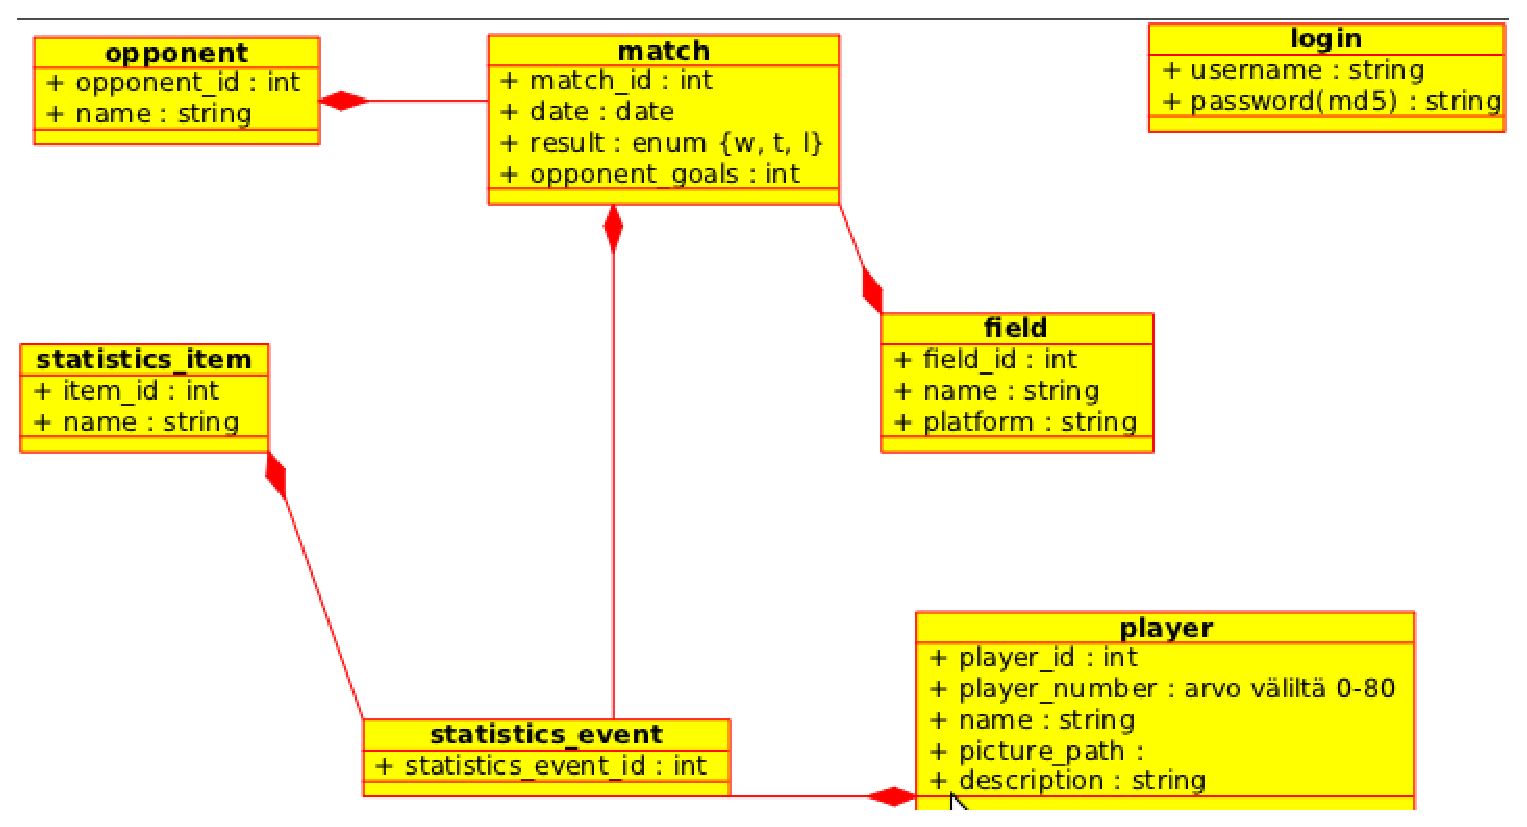
\includegraphics[width=\textwidth]{kaavio.eps}
	\end{left}
	\caption{Tietosisältökaavio}
	\label{fig:kaavio}
\end{figure}
Tietosisältökaavio näyttää ymmärrettävässä muodossa kuinka erilaiset riippuvuussuhteet yhdessä muodostavat yksilöitäviä tilastotapahtumia. Statistics\_event taulu sisältää tiedon pelaajasta, ottelusta ja tilastoartikkelista. Ottelussa voi tulla toki useita samanlaisia tilastomerkintöjä, mutta jokaista riviä yksilöi oma tunnuksensa. Tällä rakenteella kaikkea tilastoitavaa, uusia pelaajia, joukkueita ja kenttiä voidaan lisätä dynaamisesti ilman että toiminnallisuus rikkoutuisi.  Riippuvuuksien myötä voidaan selvittää niinkin spesifisiä tietoja, kuten millä pelialustalla loukkaantuminen tapahtui, ketä vastaan ja minä päivänä. Otteluiden lopputuloksetkin voidaan tuottaa helposti laskemalla maalitapahtumat statistics\_event taulusta tietyllä match\_id:llä ja vertaamalla sitä saman match\_id:n match-taulun opponent\_goals kenttään. Login taulua käytetään tässä vaiheessa vain demonstroimaan, miten johtoporras saa erilaisia näkymiä ohjelmaa käytettäessä. Jatkossa sama username-password kaksikko integroidaan jokaiselle pelaajalle.
\subsection{Käyttöliittymän rakenne} % Sub-sub-section
AC Hannes Statistics Toolin rakenne koostuu kahdesta erilaisesta näkymästä. Toinen kaikille avoin näkymä on tilasto-widget, jonka tarkoitus on olla siirrettävä ja helposti asennettava omalle kotisivulle. Tällä hetkellä se on toteuttu prototyyppimuodossaan omana sivustonaan, mutta ehkä myöhempänä ajankohtana sen voisi liittää pluginina vaikkapa wordpress sivuilleen. Widget koostuu tilastotaulusta ja suodatinvalikosta. Tilastotaulu esittää kaikkien kantaan lisättyjen tilastoartikkelien summat pelaajakohtaisina riveinä. Suodatinvalikko tarjoaa kenelle tahansa mahdollisuuden tarkastella tämän taulun tietoja järjestettynä eri tilastoartikkelin mukaan, eri ottelukohtaisia tilastoja sekä yksittäisen pelaajan tilastoja. Kaikki mahdolliset suodatinkokoonpanot ovat otettuna huomioon. Käyttäjä voi siis listata vaikkapa FC Herkulesta vastaan tehdyt maalit ottelussa FC Baggbölea vastaan. Tässä ei sinänsä ole mitään järkeä, mutta se demonstroi tilastotyökalun voimaa monipuolisuudessa.

Tilastojärjestelmän päivittäminen tapahtuu sille omistetulta sivulta, jonne on sisäänpääsy vain tietyiltä henkilöiltä. AC Hannes joukkueen tapauksessa näitä henkilöitä kuvataan sanalla johtoporras. Johtoporras on jalkapallojoukkueen osajoukko, jolla on oikeudet lisätä tilastotietoja järjestelmään. Tämä onnistuu kirjautumalla etusivulla sisään(prototyypissä username=johto password=kulta). Ilman kirjautumisen suomaa sessiodataa päivityssivu ei lataa työkalua. Päivityssivu jakautuu kahteen loogiseen osaan: tilastotapahtuma- ja resurssitaulujenhallinta osaan. Tilastotapahtumia voi lisätä järjestelmässä vain yksi kerrallaan, mutta kuitenkin usealle pelaajalle 

%----------------------------------------------------------------------------------------
%	MAJOR SECTION 1
%----------------------------------------------------------------------------------------

\section{Vaatimukset ja Käyttötapaukset} % Major section


%------------------------------------------------

\subsection{Vaatimukset} % Sub-section

\subsubsection{Subsubsection 1} % Sub-sub-section


%------------------------------------------------

\subsubsection{Subsubsection 2} % Sub-sub-section


%------------------------------------------------

\subsubsection{Subsubsection 3} % Sub-sub-section

\begin{description} % Numbered list example

\item[First] \hfill \\

\item[Second] \hfill \\

\item[Third] \hfill \\

\end{description} 

%----------------------------------------------------------------------------------------
%	MAJOR SECTION X - TEMPLATE - UNCOMMENT AND FILL IN
%----------------------------------------------------------------------------------------

%\section{Content Section}

%\subsection{Subsection 1} % Sub-section

% Content

%------------------------------------------------

%\subsection{Subsection 2} % Sub-section

% Content

%----------------------------------------------------------------------------------------
%	CONCLUSION
%----------------------------------------------------------------------------------------

\subsection{Käyttötapaukset}
\section{Loppumietelmät ja tulevat ominaisuudet} % Major section
Kokemattomuus PHP:n kanssa johti hieman kökköön toteutukseen, jota olisi tarkoitus kehittää hieman elegantimmaksi. Tarkoituksena olisi että yhä useammat urheilujoukkueet voisivat helposti asentaa kotisivuilleen AC Hannes Statistics Toolin voiman. Tiedon taitavampi käsittely mahdollistaisi esimerkiksi graafien tai muiden visuaalisten mallien helpon luomisen. Tulevaisuudessa AC Hannes Statistics Toolia laajennetaan myös android sovellukseksi, jolloin faneille voidaan tarjoilla reaaliaikaista tilastotietoa suoraan kentän laidalta.

%----------------------------------------------------------------------------------------
%	BIBLIOGRAPHY
%----------------------------------------------------------------------------------------

\begin{thebibliography}{99} % Bibliography - this is intentionally simple in this template
\end{thebibliography}

%----------------------------------------------------------------------------------------

\end{document}


